\documentclass[11pt]{article}

\usepackage{geometry}
\geometry{a4paper, portrait, margin=2cm}

\usepackage{helvet}
\renewcommand{\familydefault}{\sfdefault}

\usepackage{setspace}
\usepackage{indentfirst}
\usepackage{soul, color}
\usepackage{parskip}
\usepackage{lineno}
\usepackage{graphicx}
\usepackage[labelfont=bf]{caption}
\usepackage{float}

%opening

\begin{document}

	\begin{titlepage}
		
		\begin{center}

		\vspace*{4cm}
		\Huge
		\textbf{High Performance Computing Programming Excercises.}\\
		
		\vspace{6cm}		
			
		\large
		
		\textbf{Student:}\\
		David Bridgwood\\
		dmb2417@ic.ac.uk\\
		MRes - Computational Methods in Ecology and Evolution
		
		\end{center}
		
	\end{titlepage}
	
		
	\onehalfspacing
	\begin{flushleft}
		
		\section*{Neutral Theory Simulations}
		
			\subsection*{Question 8 - Neutral Time Series}
			
			Species Richness was plotted for a Neutral Theory simulation with no speciation over 200 generations fig.\ref{fig1}. There was an initial dramatic decrease in species richness in the earlier (first 25) generations and then a more gradual decrease until the species richness eventually reached one. This will always occur where there is no speciation as at each neutral step one individual dies and is replaced by the offspring of another, as no new species are created through speciation then eventually the system will always homogenise to a species richness of one. 
			
			\begin{figure}[H]
				\centering
				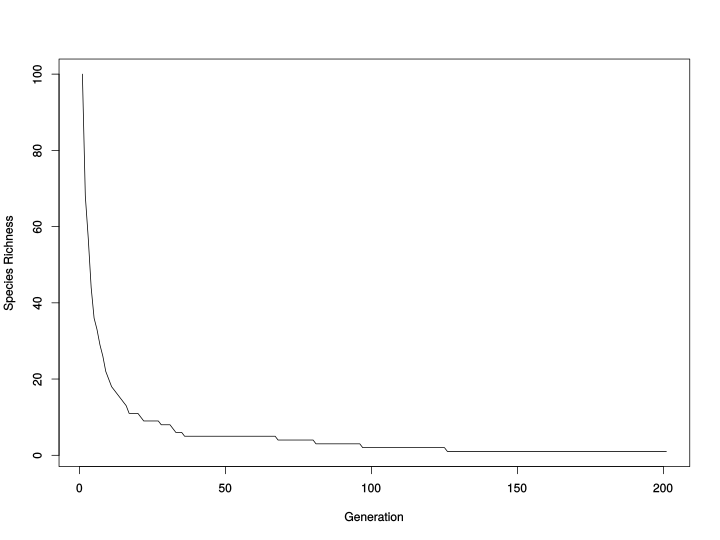
\includegraphics[width = \textwidth]{../Results/question_8.pdf}
				\caption{Species richness moving to one when under Neutral Theory simulation with no speciation. Community Size: 100, run for 200 generations.}
				\label{fig1}
			\end{figure}
						
			
			\subsection*{Question 12 - Neutral Time Series with Speciation}
			
			Species Richness was plotted for a Neutral Theory simulation with a speciation rate of 0.1 and community size of 100 for 200 generations fig.\ref{fig2}, beginning at both the maximum and minimum possible species richness'. Both initial conditions reached the same dynamic equilibria for species richness. This is because now at each neutral step there are two possible outcomes, either as before one individual dies and is replaced by the identical of another, or, there is a chance (dictated by the speciation rate) that the dying individual will be replaced by an individual from a new unique species. Given that the chance of these possibilities is identical for individuals in both simulations the dynamic equilibria they reach will be the same. 
			
			
			\begin{figure}[H]
				\begin{center}
					\centering
					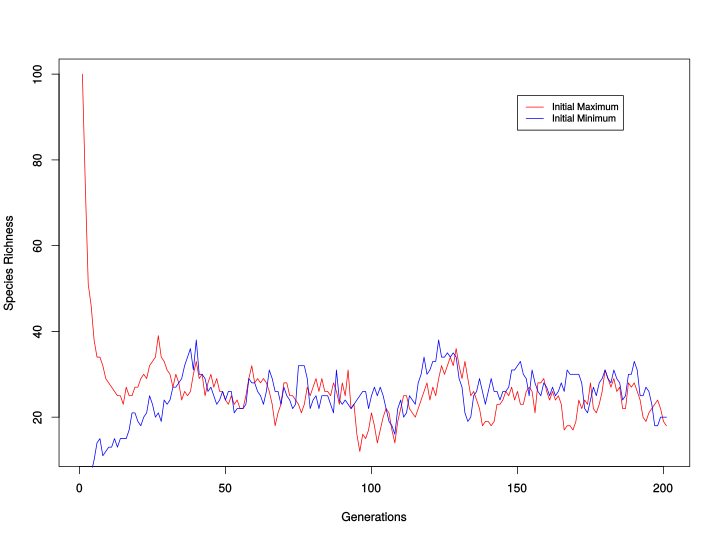
\includegraphics[width = \textwidth]{../Results/question_12.pdf}
					\caption{Species richness under Neutral Theory simulation with 0.1 probability of speciation. Community Size: 100, run for 200 generations.}
					\label{fig2}
				\end{center}
			\end{figure}
		
			\subsection*{Question 16 - Species Abundances after Neutral Theory Simulation}
			
			A Neutral Theory Simulation with a speciation rate of 0.1 and community size of 100 was run for 2000 generations with an additional 200 'burn-in generations' at the start of the simulation to ensure that the simulated community had reached equilibrium before any data was recorded. After this burn-in period species abundances were recorded every 20 generations and grouped in octaves ($2^n$ to $2^n-1$). The average number of species in these octaves is shown below fig.\ref{fig3}. 
			
			As the burn-in generations are not included in the recorded species abundances the initial conditions of the community do not matter. This is because species richness quickly reaches the same equilibrium given minimum or maximum starting richness, as was shown in question 12 fig.\ref{fig2}. 
			
			
			\begin{figure}[H]
				\centering
				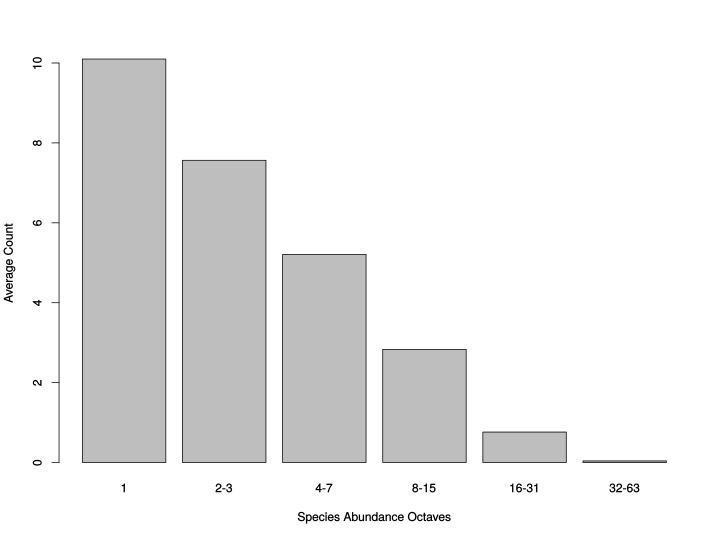
\includegraphics[width = \textwidth]{../Results/question_16.pdf}
				\caption{Distribution of Species Abundance after a Neutral Theory Simulation with speciation rate 0.1 and community size 100, run for 2000 generations.}
				\label{fig3}
			\end{figure}
				
			\subsection*{Challenge Question A}
			
			A Neutral Theory Simulation with a speciation rate of 0.1 and community size of 100 was run for 1000 generations, the species richness of the community was recorded at each iteration of the simulation (every generation). This simulation was repeated 100 times for both at initial maximum and initial minimum starting richness as the starting community. The mean species richness was plotted against generations with 97.2\% confidence limits fig.\ref{ca}. From this it is clear that the community reached dynamic equilibrium by approximately generation 50, and therefore a much shorter burn in period could have been used in question 16.
			
			
			\begin{figure}[H]
				\centering
				\includegraphics[width = \textwidth]{../Results/challenge_A.pdf}
				\caption{Average species richness from 100 repeated simulations for the first 1000 generations. Community size of 100 starting at both maximum and minimum initial richness and a speciation rate of 0.1. 97.2\% confidence intervals shown. Vertical line at generation 50 - approximately where dynamic equilibrium is reached.}
				\label{ca}
			\end{figure}
		
	\end{flushleft}
	
\end{document}